\section{习题参考答案}
\subsection*{一、填空题}
\begin{enumerate}
    \item 边长为$a$的正方形的四个顶点上放置如图所示 \ref{Fig:46} 的点电荷, 则中心$o$处场强为\anl{$\frac{\sqrt{2}q}{2\pi \epsilon_0 a^2}\vec{j}$}.
    \begin{figure}[H]
        \centering
        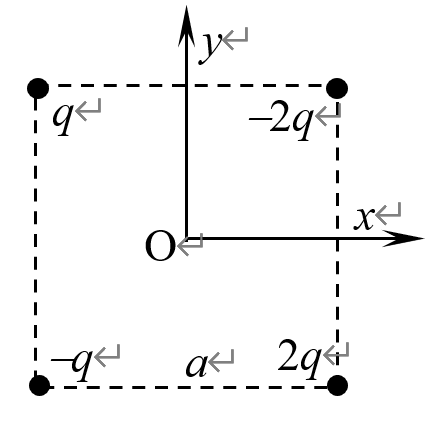
\includegraphics[width=0.15\textheight]{fig46}
        \caption{如图.}\label{Fig:46}
    \end{figure}
    \begin{note}
    \textcolor{red}{分别将每个点电荷在$O$点产生的电场强度分解到$x$和$y$方向,根据电场叠加原理及几何关系可得$O$点电场强度为$\frac{\sqrt{2}q}{2\pi \epsilon_0 a^2}\vec{j}$}
    \end{note}
    \item 在点电荷系的电场中, 任一点的电场强度等于\underline{各点电荷单
    独存在时在该点产生场强}\\ \underline{的矢量和}, 这称为电场强度叠加原理.
    \item 正方形的两对角上, 各置电荷$Q$, 在其余两对角上各置电荷$q$, 若$Q$所受合力为零,则$Q$与$q$的大小关系为\anl{$Q=-2\sqrt{2}$}.
    \begin{note}
        \begin{figure}[H]
            \begin{minipage}[H]{0.6\linewidth}
                \begin{table}[H]
                    \hspace*{1.5cm}如图受力分析,设正方形边长为$a$,\\
                    \hspace*{1.5cm}欲使$Q$受合外力为零,则$q$与$Q$电性相反, \\
                    \hspace*{1.5cm}利用库仑定律得:\par
                    \vspace*{0.1cm}
                    \hspace*{1.5cm}$\frac{Q^2}{4\pi \varepsilon_0 (\sqrt{2}a)^2}=\sqrt{2}\frac{-qQ}{4\pi \varepsilon_0 a^2}$, $\therefore Q=-2\sqrt{2}q$
                \end{table}  
            \end{minipage}
            \begin{minipage}[H]{0.3\linewidth}
                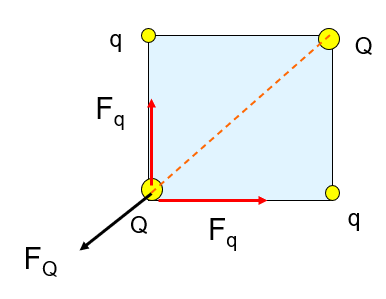
\includegraphics[width=1\textwidth]{ans29}
            \end{minipage}
        \end{figure}
    \end{note}
    \item   如图所示 \ref{Fig:49}, 真空中有两个点电荷, 带电量分别为$Q$和$-Q$, 相距$2R$。若以负电荷
    所在处$O$点为中心, 以$R$为半径作高斯球面$S$, 则通过该球面的电场强度通量$\varPhi_e$=\anl{$-Q/\varepsilon_0$}. 
    \begin{figure}[H]
        \centering
        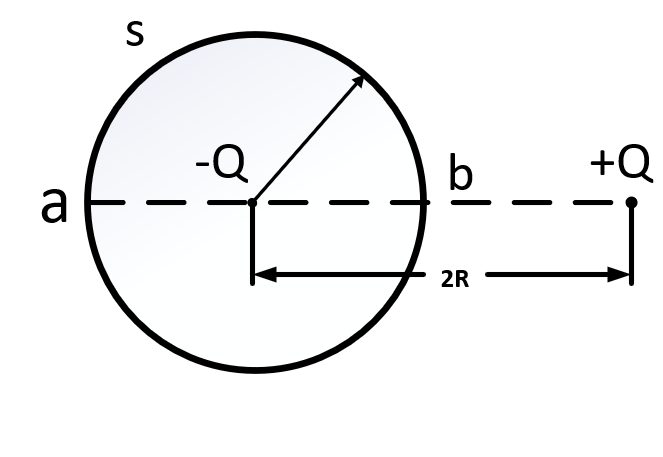
\includegraphics[width=0.15\textheight]{fig49}
        \caption{如图.}\label{Fig:49}
    \end{figure}
    \begin{note}
        \textcolor{red}{根据高斯定理,通过任一闭合面的电场强度通量等于该闭合曲面所包围的电荷的代数和乘以$1/\varepsilon_0$
        }
    \end{note}
    \item 如图所示\ref{Fig:50}, 在场强为$E$的均匀电场中取一半球面, 其半径为$r$, 电场强度的方向与半球面的对称轴平行. 则通过这个半球面的电通量$\varPhi_e$=\anl{$E\pi R^2$}.
    \begin{figure}[H]
        \centering
        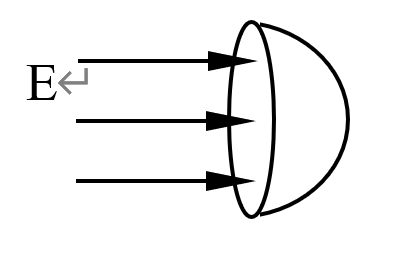
\includegraphics[width=0.15\textheight]{fig50}
        \caption{如图.}\label{Fig:50}
    \end{figure}
    \begin{note}
        \textcolor{red}{根据电通量定义式, $\varPhi_e=\int_S \vec{E}\cdot \dd \vec{S}$,由于半球面在E垂直方向的投影为圆,其面积为~$\pi R^2$
        }
    \end{note}
    \item 一点电荷$q$位于一位立方体中心, 立方体边长为$a$, 则通过立方体每个表面的$\vec{E}$的通量\anl{$9/6 \varepsilon_0$};若把这电荷移到立方体的一个顶角上, 这时通过电荷所在顶角的三个面$\vec{E}$的通量是\anl{0}, 通过立方体另外三个面的$\vec{E}$的通量是\anl{$q/8\varepsilon_0$}.
    \begin{note}
        \textcolor{red}{对于立方体,根据高斯定理~$\varPhi_e=\vec{E}\cdot\vec{S}=q/\varepsilon_0$, 则通过每个表明的通量为~$\vec{E}\cdot (\vec{S}/6)=q/6\varepsilon_0$.}\ \ 
        \textcolor{red}{若把电荷移动到一个顶角上时,则穿过电荷所在顶角的三个表明的电场为零,故通量为零.
        }\ \ 
        \textcolor{red}{因为一个顶角上的电荷可供八个立方体所共有,故通过任意一个立方体的通量为~$q/8\varepsilon_0$}
    \end{note}
    \item 一均匀静电场, 场强$\vec{E}=(400\vec{i}+600\vec{j})v\cdot m^{-1}$, 则点$a(3, 2)$和点$b(1, 0)$之间的电势差$U_{ab}$=\anl{$-2000V$}.
    \begin{note}
        \textcolor{red}{$U_{ab}=\int_a^b \vec{E}\cdot \mathrm{d} \vec{l}=\vec{E}\cdot \vec{l}_ab=(400\vec{i}+600\vec{j})\cdot (-2\vec{i}-2\vec{j})=-2000V$}
    \end{note}
    \item 如图所示\ref{Fig:52}, 半径为$R$的均匀带电球面, 总电荷为$Q$, 设无穷远处的电势为零, 则球内距离球心为$r$的$P$点处的电势$U$=\anl{$\frac{Q}{4\pi \varepsilon_0 R}$}. 
    \begin{figure}[H]
        \centering
        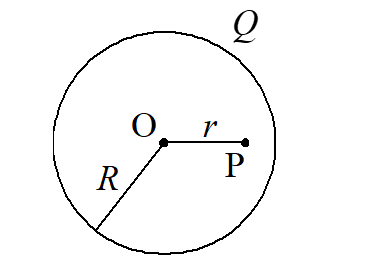
\includegraphics[width=0.15\textheight]{fig52}
        \caption{如图.}\label{Fig:52}
    \end{figure}
    \begin{note}
        如图:
        \begin{figure}[H]
            \centering
            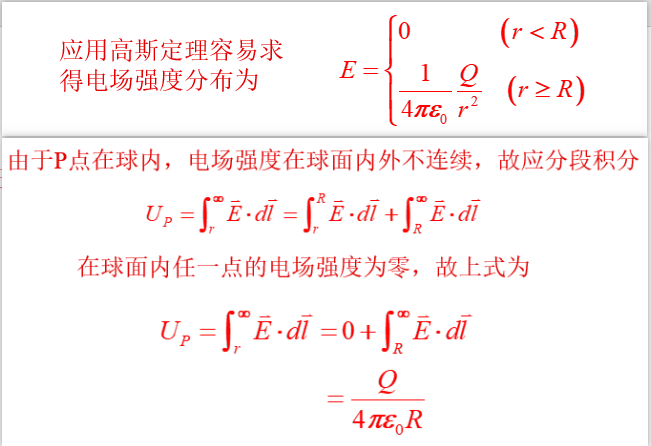
\includegraphics[width=0.4\textheight]{ans30}
        \end{figure}
    \end{note}
    \item 一“无限长”均匀带电直线沿$Z$轴放置, 线外某区域的电势表达式为$U=A\mathrm{ln}(x2+y2)$, 式中$A$为常数, 该区域电场强度的两个分量为: $E_x$=\underline{$-\frac{2Ax}{x^2+y^2}$}, $E_y$=\underline{$-\frac{2Ay}{x^2+y^2}$}.
    \begin{note}
        \textcolor{red}{根据电场与电势的关系:$\vec{E}=-\Delta U=-\left(\frac{\partial U}{\partial x}\vec{i}+\frac{\partial U}{\partial y}\vec{j}+\frac{\partial U}{\partial z}\vec{k}\right)$}\par
        \textcolor{red}{$\therefore E_x = -\frac{\partial U}{\partial x}=-\frac{2Ax}{x^2+y^2}$, \ $E_y = -\frac{\partial U}{\partial y}=-\frac{2Ay}{x^2+y^2}$}
    \end{note}
\end{enumerate}
\subsection*{二、选择题}
\begin{enumerate}
    \item 如图所示 \ref{Fig:47}, 一电偶极子, 正点电荷在坐标$(a,0)$处, 负点电荷在坐标$(-a,0)$处, $P$点是$x$轴上的一点, 坐标为$(x,0)$. 当$x>>a$时, 该点场强的大小为(~D~)
    \fourch{$\frac{q}{4\pi\varepsilon_0x}$;}{$\frac{q}{4\pi\varepsilon_0x^2}$;}{$\frac{qa}{2\pi\varepsilon_0x^3}$}{$\frac{qa}{\pi\varepsilon_0x^3}$.}
    \begin{figure}[H]
        \centering
        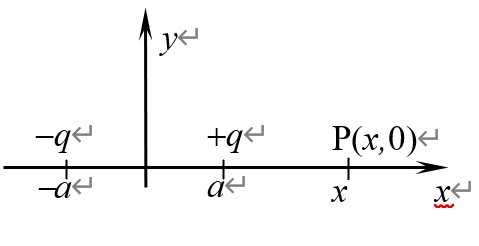
\includegraphics[width=0.15\textheight]{fig47}
        \caption{如图.}\label{Fig:47}
    \end{figure}
    \begin{note}
        \begin{figure}[H]
        \centering
        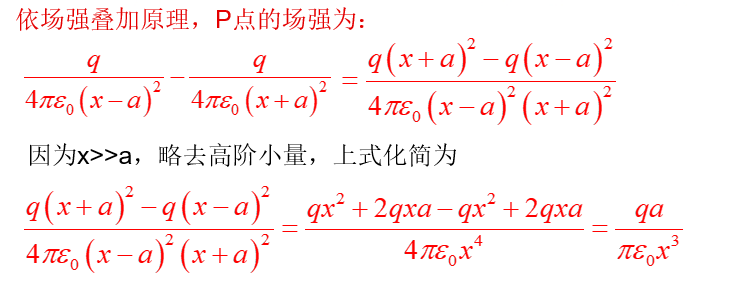
\includegraphics[width=0.4\textheight]{ans31} 
    \end{figure}
    \end{note}
    \item 真空中面积为$S$, 间距$d$的两平行板$S>>d_2$, 均匀带等量异号电荷+q和-q, 忽略边缘效应, 则两板间相互作用力的大小是(~C~).
    \twoch{$\frac{q^2}{(4\pi\varepsilon_0d^2)}$; }{$\frac{q^2}{(\varepsilon_0 s)}$;}{$\frac{q^2}{(2\varepsilon_0s)}$;}{$\frac{q^2}{(2\pi\varepsilon_0d^2)}$.}
    \begin{note}
        \textcolor{red}{解:由例7.7结论知,均匀带点“无限大”平面外任意一点处电场强度为:$E=\frac{\sigma}{2\varepsilon_0}$}\par
        \textcolor{red}{则两板间相互作用力的大小为~$F_{q+}=q_+E_\_=\frac{q\sigma}{2\varepsilon_0}=\frac{q}{2\varepsilon_0}\cdot\frac{q}{s}=\frac{q^2}{2\varepsilon_0 s}$        }
    \end{note}
    \item  下列哪一种说法正确 (~A~)
    \onech{电场线上任意一点的切线方向, 代表这点的电场强度的方向;}{在某一点电荷附近的任一点, 若没放试验电荷, 则这点的电场强度为零;}{若把质量为$m$的点电荷$q$放在一电场中, 由静止状态释放, 电荷一定沿电场线运动;}{电荷在电场中某点受到的电场力很大, 该点的电场强度一定很大.}
    \begin{note}
        \textcolor{red}{B:电荷周围存在电场,无关试验电荷是否存在\quad C:  应考虑重力作用,故不沿电场线方向\quad D:  电场力的大小与所放电荷的电量也有关
        }
    \end{note}
    \item 关于高斯定理的理解有下面几种说法, 其中正确的是(~D~)
    \onech{如果高斯面上$\vec{E}$处处为零, 则该面内必无电荷;}{如果高斯面内无电荷, 则高斯面上$\vec{E}$处处为零;}{如果高斯面上$\vec{e}$处处不为零, 则高斯面内必有电荷;}{如果高斯面内有净电荷, 则通过高斯面的电场强度通量必不为零.}
    \begin{note}
        \textcolor{red}{A:高斯面内有等电量异号电荷时,高斯面上电场也处处为零。\ B:高斯面外电荷可在高斯面上产生电场,使高斯面上的电场     
        强度可不为零,但通过高斯面的总通量为零。\ C:同B
}
    \end{note}
    \item 下述带电体系的场强分布可能用高斯定理来计算的是(~D~)
    \twoch{均匀带电圆板}{有限长均匀带电棒}{电偶极子}{带电介质球(电荷体密度是离球心距离$r$的函数)}
    \begin{note}
        \textcolor{red}{应用高斯定理计算场强分布时,要求带电体系产生的电场在空间分布应具有对称性,可忽略边缘效应。故选D
        }
    \end{note}
    \item 已知某电场的电场线分布情况如图所示\ref{Fig:53}. 现观察到一负电荷从$M$点移到$N$点. 有人根据这个图作出下列几点结论, 其中正确的是(~C~)
    \twoch{电场强度$E_M$<$E_N$}{电势$U_M$<$U_N$}{电势能$W_M$<$W_N$}{电场力的功$A>0$}
    \begin{figure}[H]
        \centering
        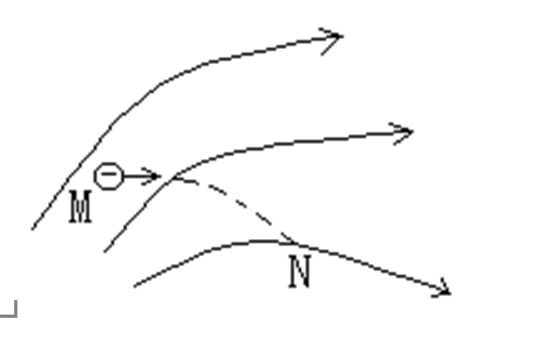
\includegraphics[width=0.15\textheight]{fig53}
        \caption{如图.}\label{Fig:53}
    \end{figure}
    \begin{note}
        \textcolor{red}{A: 电场线密集的地方电场强度大, 故$E_M>E_N$。\ \ B:沿电场线方向,电势降低,故$U_M>U_N$.\ \ C:由图知,负电荷从$M$点移动到$N$点过程中克服电场力做     
        功,故电场力做负功,$A<0$。\ \ 电场力做负功,电势能增加,故~C~正确.
        }
    \end{note}
    \item 如图所示\ref{Fig:54}, 下面表述中正确的是(~C~)
    \twoch{$E_A$>$E_B$>$E_C$, $U_A$>$U_B$>$U_C$}{$E_A$<$E_B$<$E_C$, $U_A$>$U_B$>$U_C$}{$E_A$>$E_B$>$E_C$, $U_A$<$U_B$<$U_C$}{$E_A$<$E_B$<$E_C$, $U_A$<$U_B$<$U_C$}
    \begin{figure}[H]
        \centering
        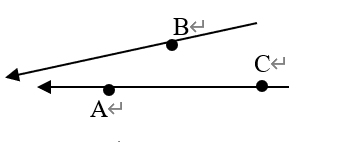
\includegraphics[width=0.15\textheight]{fig54}
        \caption{如图.}\label{Fig:54}
    \end{figure}
    \begin{note}
        \textcolor{red}{电场线越密集,电场强度越大;沿电场线方向,电势降低
        }
    \end{note}
    \item 下列关于静电场的说法中, 正确的是(~D~)
    \onech{电势高的地方场强就大}{带正电的物体电势一定是正的}{场强为零的地方电势一定为零}{电场线与等势面一定处处正交}
    \begin{note}
        \textcolor{red}{A: 匀强电场沿电场线方向电势降低,但场强不变\ \ B: 与电势零点选取有关\ \ C: 带点球面内部场强为零,但电势可以不为零}
    \end{note}
\end{enumerate}
\subsection*{三、计算题}
\begin{enumerate}
    \item 如图 \ref{Fig:48}, 内半径为$R_1$, 外半径为$R_2$的环形薄板均匀带电, 电荷面密度为$\sigma$, 求: 中垂线上任一$P$点的场强及环心处0点的场强.
    \begin{figure}[H]
        \centering
        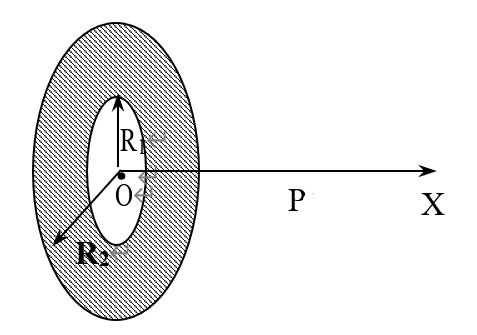
\includegraphics[width=0.15\textheight]{fig48}
        \caption{如图.}\label{Fig:48}
    \end{figure}
    \begin{solution}
        如图:
        \begin{figure}[H]
            \centering
            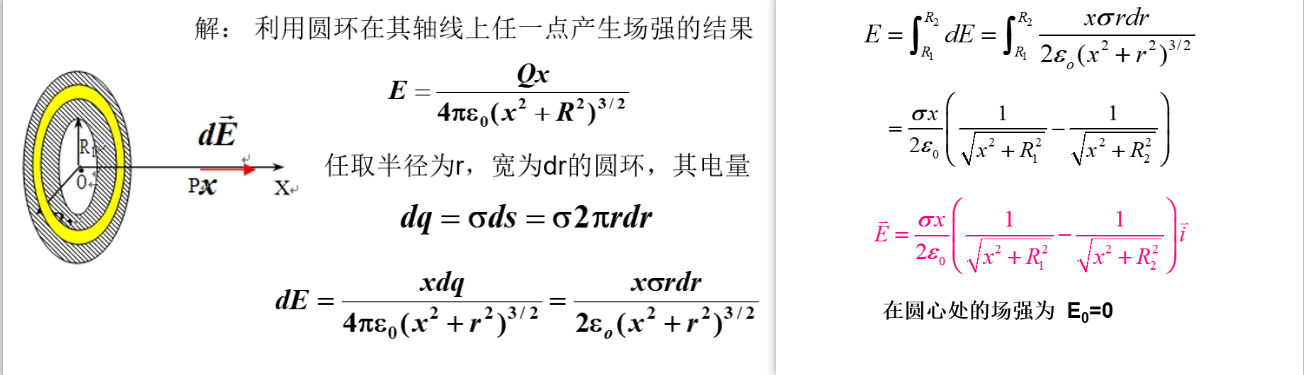
\includegraphics[width=0.55\textheight]{ans32}
        \end{figure}
    \end{solution}
    \item 如图 \ref{Fig:51}, 无限长均匀带电圆柱体,电荷体密度为$\rho$, 半径为$R$, 求柱体内外的场强分布.
    \begin{figure}[H]
        \centering
        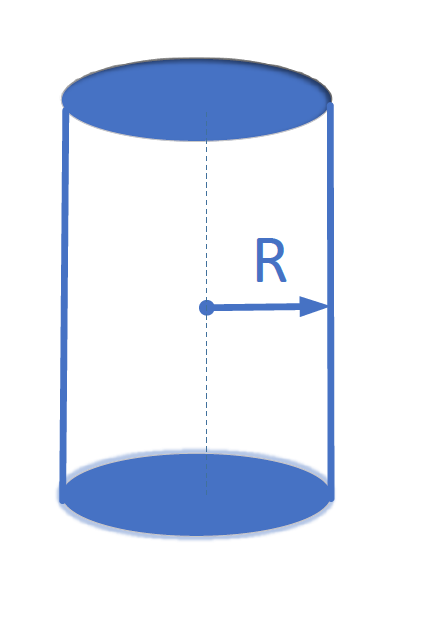
\includegraphics[width=0.15\textheight]{fig51}
        \caption{如图.}\label{Fig:51}
    \end{figure}
    \begin{solution}
        如图:
        \begin{figure}[H]
            \centering
            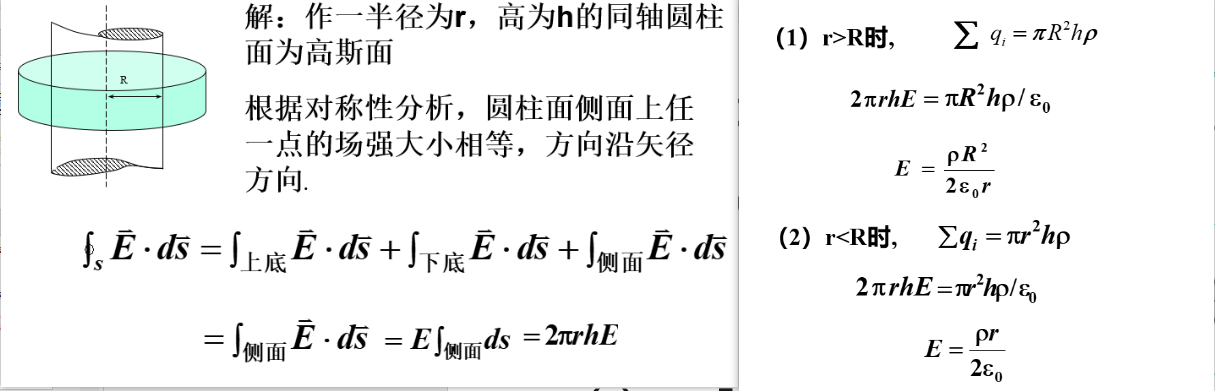
\includegraphics[width=0.55\textheight]{ans33}
        \end{figure}
    \end{solution}
    \item 如图 \ref{Fig:55}, 球壳的内半径为$a$, 外半径为$b$, 壳体内均匀带电, 电荷体密度为$\rho$, 求: 空间的场强和电势分布.
    \begin{figure}[H]
        \centering
        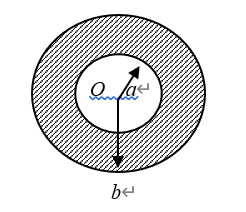
\includegraphics[width=0.15\textheight]{fig55}
        \caption{如图.}\label{Fig:55}
    \end{figure}
    \begin{solution}
        如图:
        \begin{figure}[H]
            \centering
            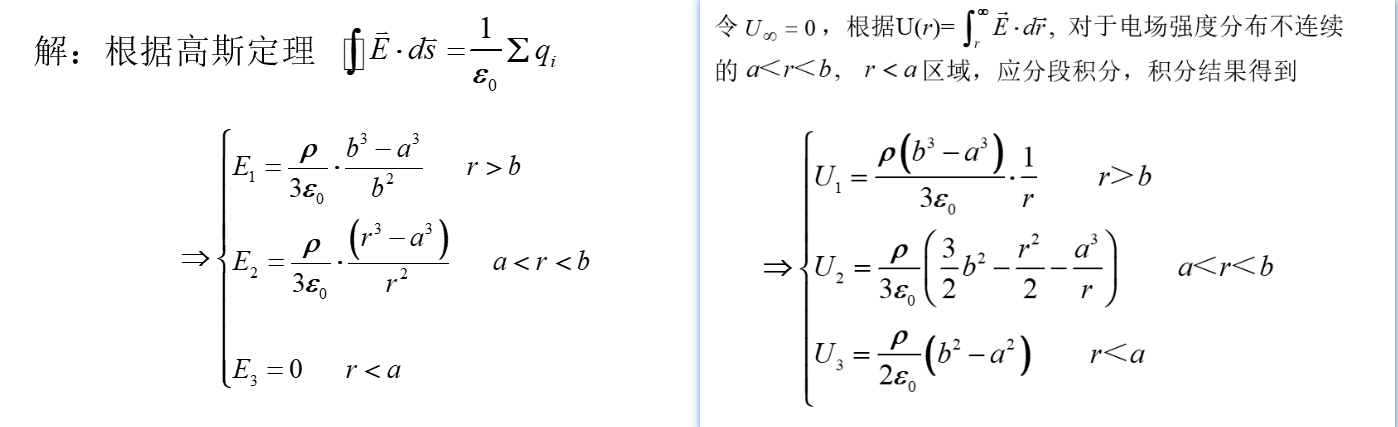
\includegraphics[width=0.55\textheight]{ans34}
        \end{figure}
    \end{solution}
\end{enumerate}